\section{Implementación y control de versiones}

\subsection{Introducción}

\quad En esta parte se presentan las diferentes implementaciones necesarias, así como un control de versiones de la aplicación en la que desmenuzaremos las diferentes versiones. \\

\quad Llevar un control de versiones es esencial como desarrollador, por lo que para este fin utilizo la página \textit{github}, y como herramienta secundaria para la gestión del repositorio, utilizo \textit{GitKraken}. Para el desarrollo de esta aplicación se ha seguido el paradigma de \textit{GitFlow} a la hora del control de versiones con el repositorio.\\
 
\subsection{GitFlow}
\subsubsection{¿Qué es GitFlow?}

\quad Gitflow es un diseño de flujo de trabajo Git que se publicó por primera vez y se hizo popular por \textit{Vincent Driessen} en \textit{nvie}. El flujo de trabajo de Gitflow define un modelo de ramificación estricto diseñado en torno al lanzamiento del proyecto. Esto proporciona un marco robusto para gestionar proyectos más grandes.\\

\quad Gitflow es ideal para proyectos que tienen un ciclo de lanzamiento programado, pues este flujo de trabajo no agrega nuevos conceptos o comandos más allá de lo que se requiere para el Flujo de trabajo de la rama de funciones, si no que asigna roles muy específicos a diferentes ramas y define cómo y cuándo deben interactuar. Además de las ramas de características, utiliza ramas individuales para preparar, mantener y grabar lanzamientos. Por supuesto, también puede aprovechar todos los beneficios del flujo de trabajo de Branch Branch: solicitudes de extracción, experimentos aislados y una colaboración más eficiente.\\ 

\subsubsection{¿Cómo funciona?}

\subsubsubsection{Ramas Develop \& Master}

\quad En lugar de una sola rama, este flujo de trabajo usa dos ramas para registrar el historial del proyecto.\\ 

\quad La rama \textit{master} almacena el historial de lanzamiento oficial, y la rama \textit{develop} sirve como una rama de integración de características. También es conveniente etiquetar todos los commits en master con un número de versión.\\

\begin{figure}[htb]
	\centering
	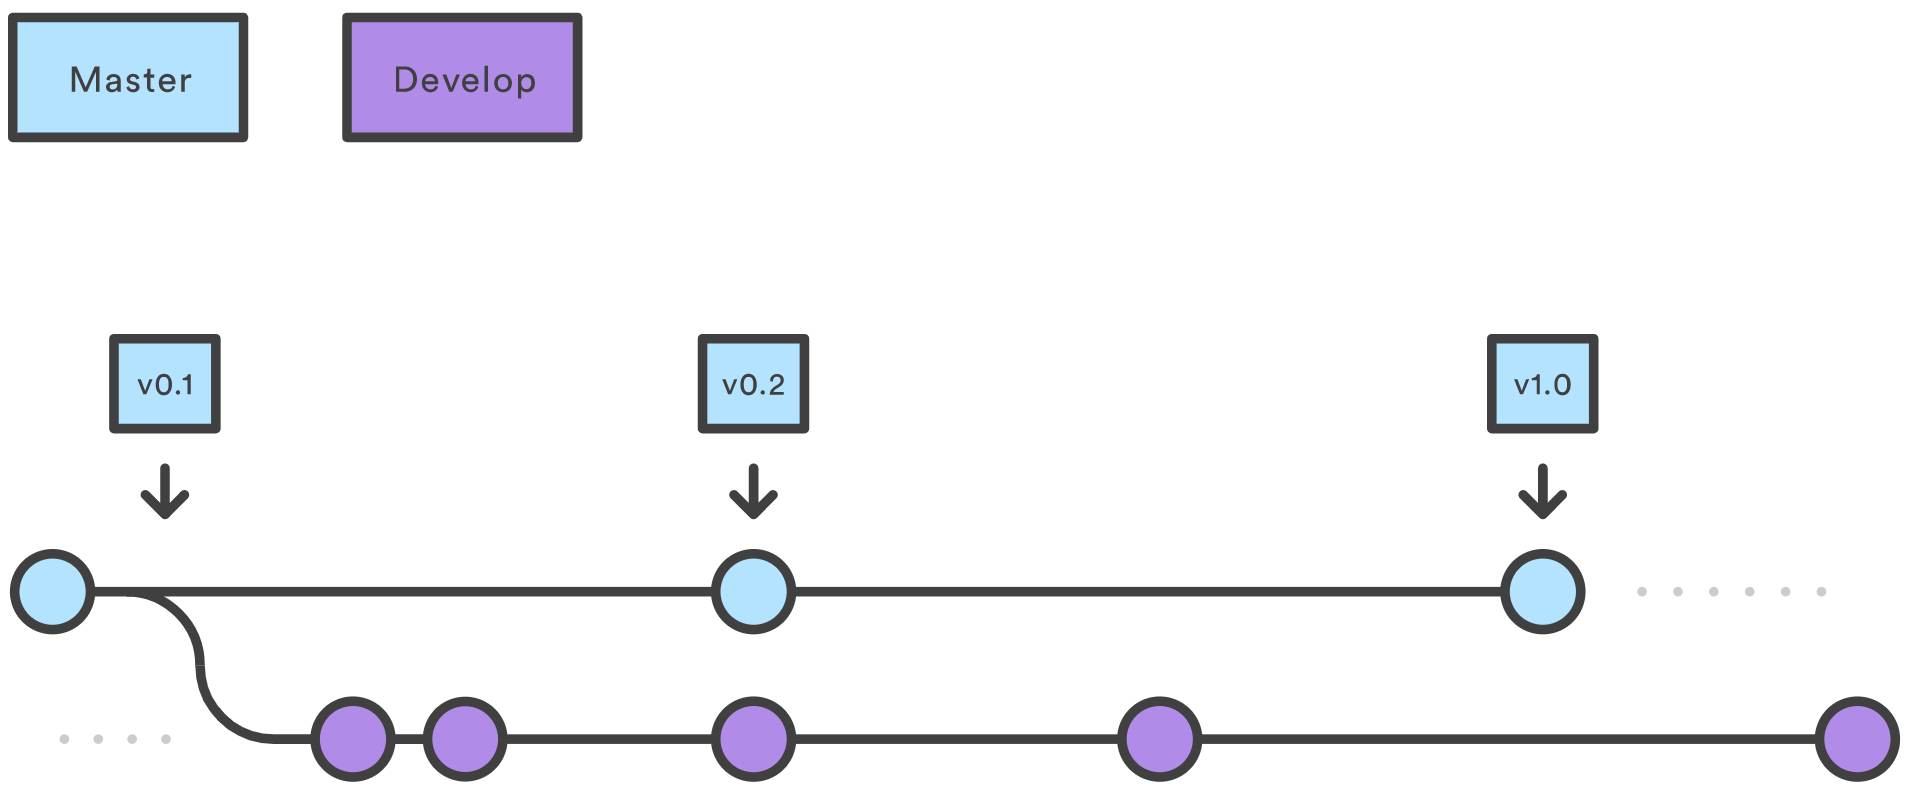
\includegraphics[width=0.75\textwidth]{./imagenes/master-dev}
	\caption{Ramas Develop y Master}
\end{figure}

\subsubsubsection{Ramas Feature}

\quad Cada nueva feature debe residir en su propia rama, que se puede enviar al repositorio central como respaldo/colaboración.\\

\quad En lugar de bifurcarse de master, las features usan el desarrollo como su rama principal, de forma que cuando se completa una característica, se fusiona nuevamente en develop. Las características nunca deberían interactuar directamente con el maestro.\\

\begin{figure}[htb]
	\centering
	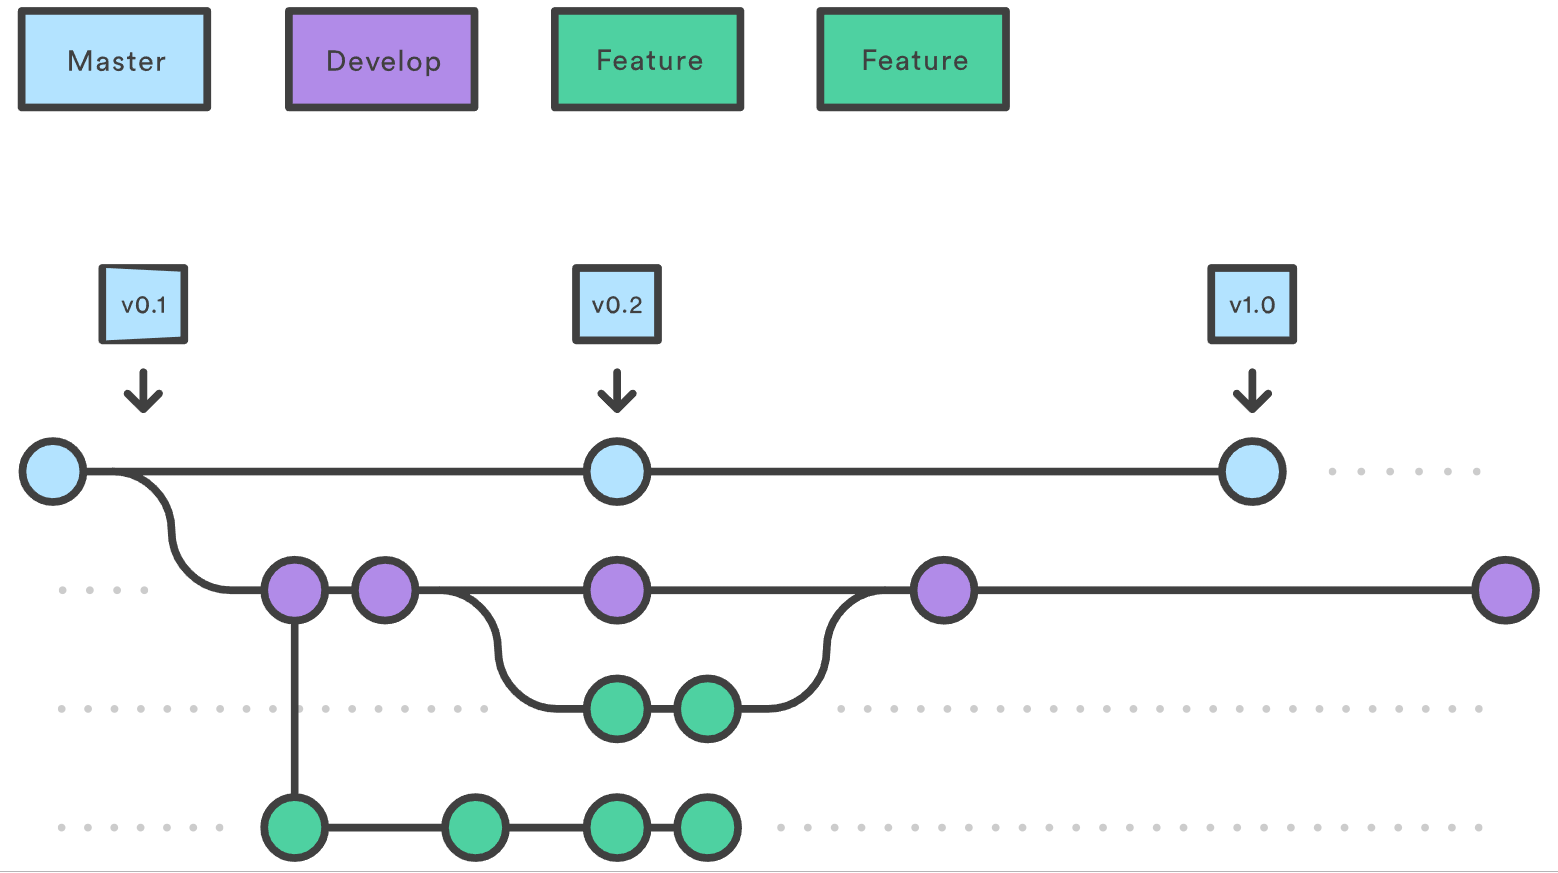
\includegraphics[width=1\textwidth]{./imagenes/feature}
	\caption{Rama feature}
\end{figure}

\subsubsubsection{Ramas Release}

\quad Una vez que el desarrollo ha adquirido suficientes características para un lanzamiento,  bifurca una rama de release fuera del desarrollo. La creación de esta rama inicia el siguiente ciclo de lanzamiento, por lo que no se pueden agregar nuevas características después de este punto. Solo las correcciones de errores, la generación de documentación y otras tareas orientadas a la versión deben ir en esta rama.\\ 

\quad Una vez que está listo para enviar, la release se fusiona en master y se etiqueta con un número de versión. Además, debe fusionarse nuevamente en el desarrollo, que puede haber progresado desde que se inició el lanzamiento.\\

\begin{figure}[htb]
	\centering
	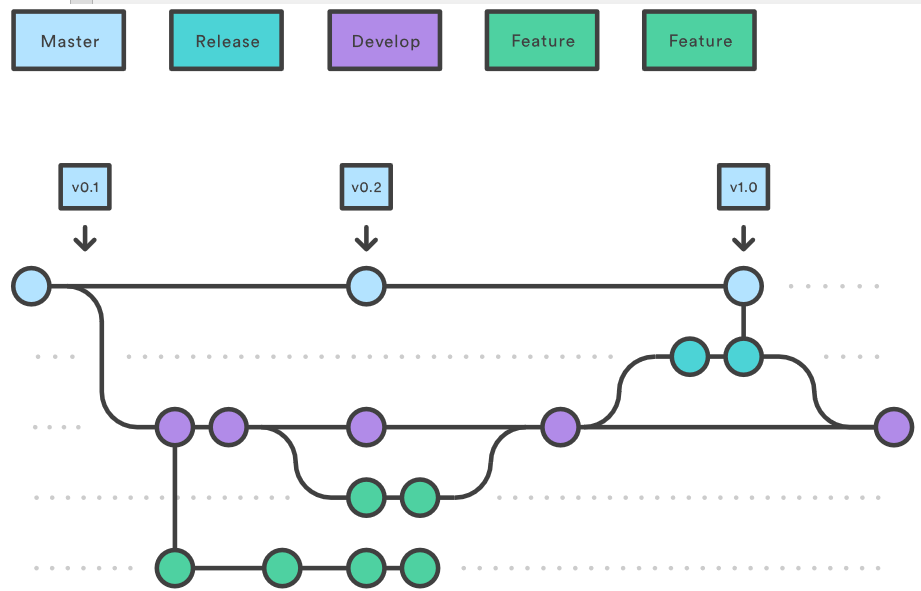
\includegraphics[width=1\textwidth]{./imagenes/release}
	\caption{Rama release}
\end{figure}

\subsubsubsection{Ramas Hotfix}

\quad Las ramas de mantenimiento o "hotfix" se utilizan para parchear rápidamente las versiones de producción.\\

\quad Las ramificaciones de revisión son muy parecidas a las ramificaciones de lanzamiento y ramificaciones de características, excepto que se basan en master en lugar de develop.\\

\quad Esta es la única rama que debe bifurcarse directamente de master, y tan pronto como se complete la corrección, debe fusionarse tanto en master como en develop (o en la rama de la versión actual), y master debe etiquetarse con un número de versión actualizado.\\

\begin{figure}[htb]
	\centering
	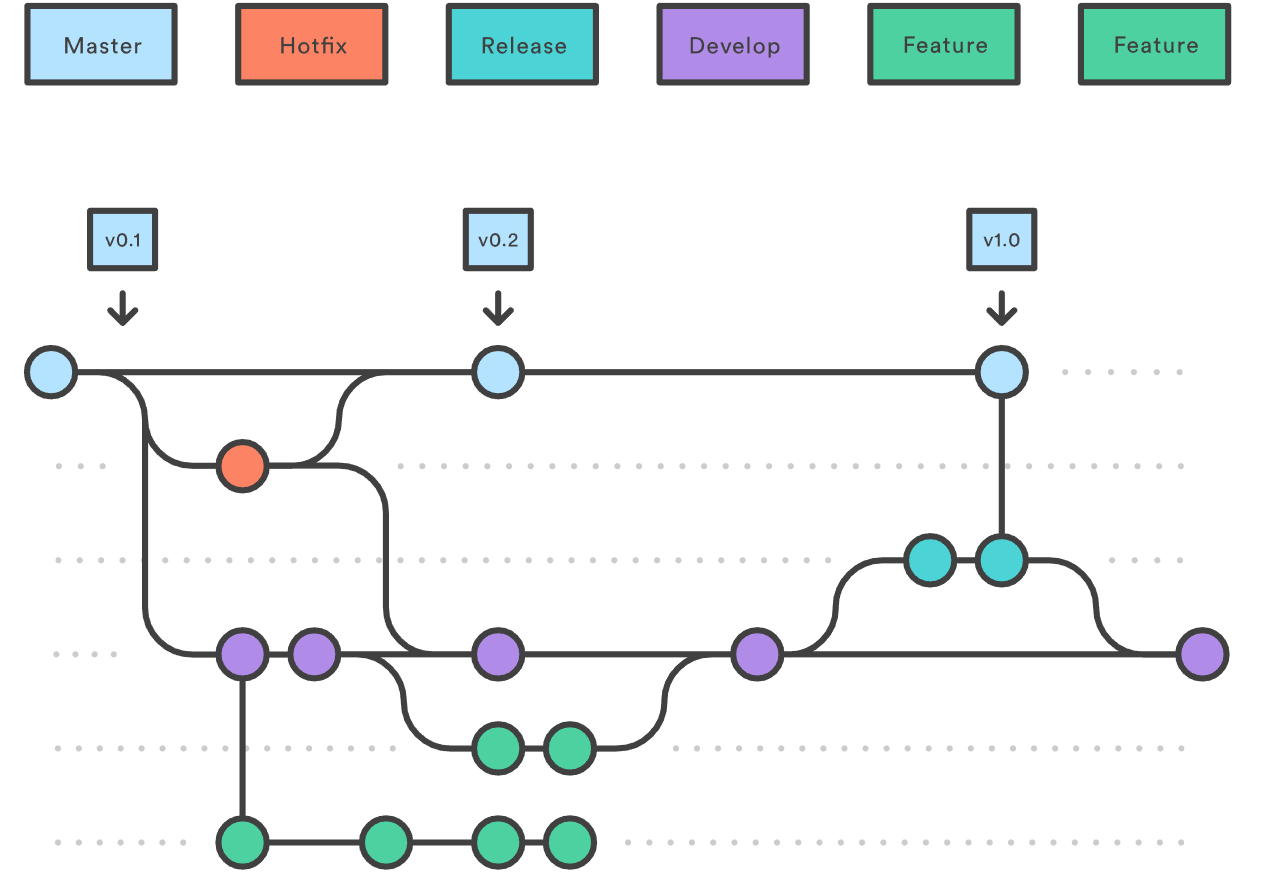
\includegraphics[width=0.6\textwidth]{./imagenes/hotfix}
	\caption{Rama hotfix}
\end{figure}

\subsection{Control de versiones}

\quad A continuación, se presenta el árbol de desarrollo de la aplicación en las que se ve un resumen de las modificaciones:

\begin{figure}[htb]
	\centering
	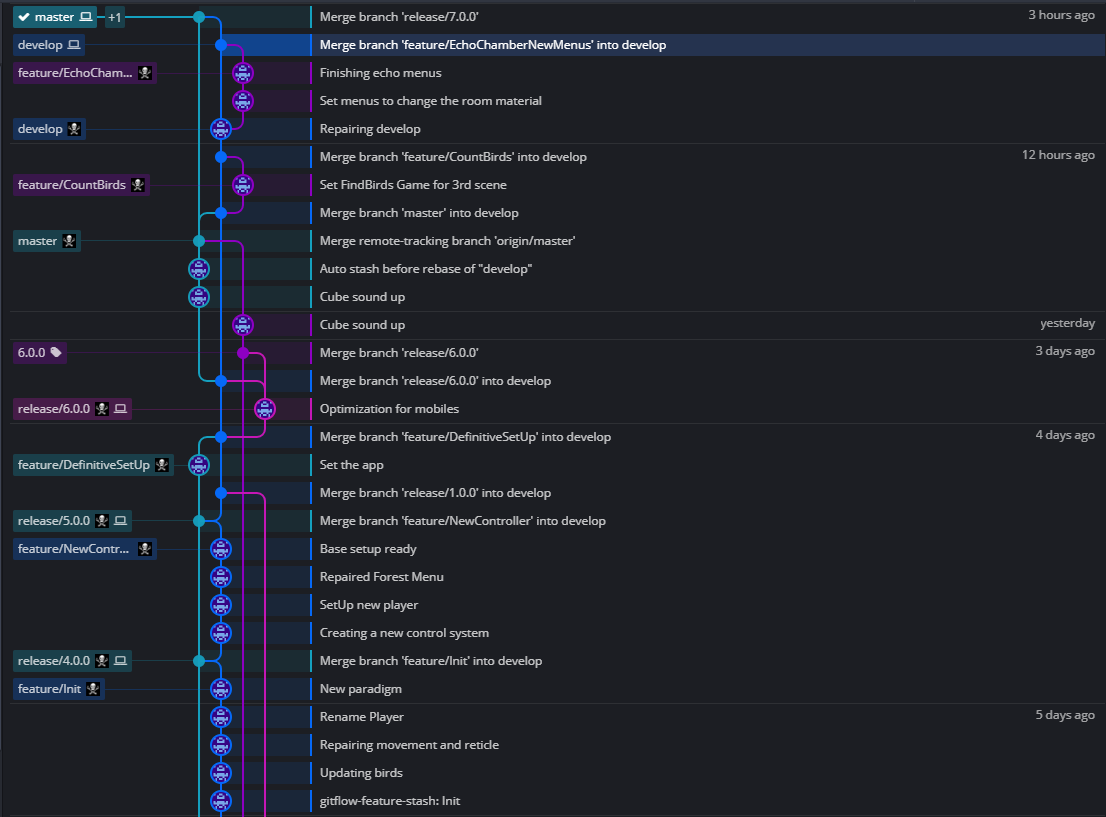
\includegraphics[width=0.6\textwidth]{./imagenes/git-tree1}
	\caption{Parte superior del gitTree}
\end{figure}

\begin{figure}[htb]
	\centering
	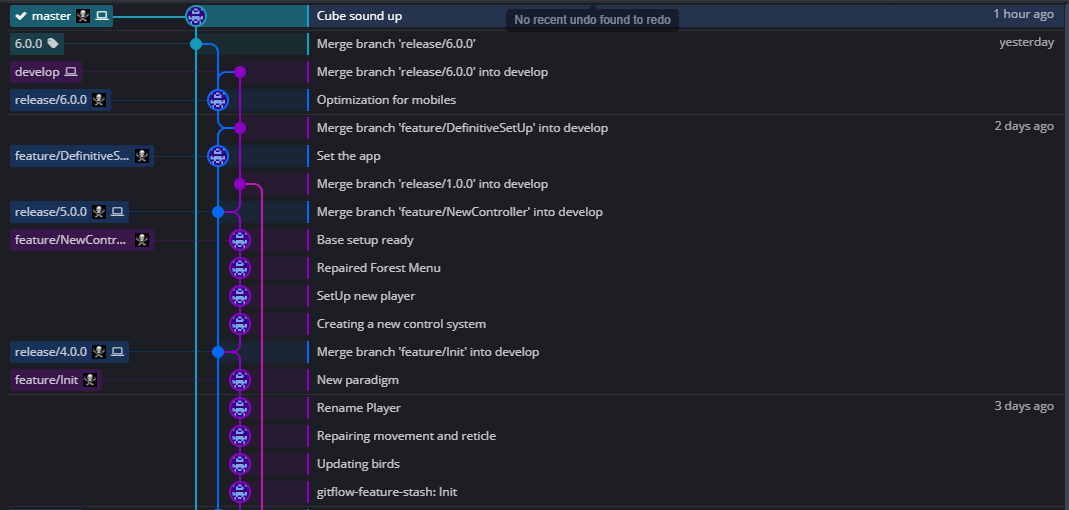
\includegraphics[width=0.6\textwidth]{./imagenes/git-tree2}
	\caption{Parte inferior del gitTree}
\end{figure}

\subsubsection{Cambios en el paradigma de interacción del usuario}

\quad El desarrollo de una aplicación no es ni mucho menos algo estático que sigue estrictamente los pasos definidos al inicio de éste durante la planificación. Un buen desarrollo debe saber adaptarse a requisitos que pudieron no tenerse en un principio.\\

\quad Este es el caso de la aplicación aqui presentada, de forma que me dispongo a enumerar unos cuantos cambios que surgieron a lo largo del desarrollo y que merecente ser resaltados por encima de los demás:

\begin{itemize}
	\item En la versión 5.0.0, desecho un control del movimiento del personaje basado en mando por un control basado únicamente en los que el cardboard nos presenta, pasando el botón de pantalla a a haber que el personaje se mueva hacia adelante, y las interacciones con elementos de las escenas presentadas con un cargador de tiempo. Este cambio surge al plantearme facilitar el uso para el usuario, al no depender de otro dispositivo externo, en este caso un mando.
	\item En la versión 6.0.0 la reticula de carga pasa a ser la propia reticula puntero que utiliza. Esto se realiza con la idea de evitar que la superposición de ambas retículas pueda marear al usuarion cuando la de carga entra en escena.
	\item  En la versión 6.0.0 se aplica oclussion culling en la escena del bosque. Esto se hace para reducir su carga y así maximizar los frames de la escena.
\end{itemize}

\subsection{Implementación general: setUp de la aplicación}

\quad El trabajo de esta aplicación se ha desarrollado con Unity 2018.4.6f1. Esto se ha hecho así debido a que el hub de Unity determinaba que esta era la última versión estable de la aplicación en el momento del inicio de la programación de este proyecto.\\

\quad Deberemos configurar también la sdk para que Unity pueda trabajar. Normalmente si ya se tiene la sdk de android instalada, Unity la reconocerá sin necesidad de añadirla manualmente.\\

\quad Debemos tener en cuenta que, en "Edit>Project Settings", debemos activar la casilla \textit{Virtual Reality Supported} de XR Settings para android en el "Player", y fijar en la pestaña "Other Settings" el \textit{Minimum API Leve} a nivel 19.\\

\subsubsection{Paquetes a descargar y assets gratuitos}

\quad Los paquetes que necesitaremos para poder utilizar la tecnología necesaria en Unity son:

\begin{itemize}
	\item ResonaceAudioForUnity\_<versión\_deseada>.unitypackage
	\item GoogleVRForUnity\_<versión\_deseada>.unitypackage
\end{itemize}

\quad Para instalar un paquete, introduciremos el paquete en cuestión desde la pestaña "Assets>Import Package>Custom Package".\\

\quad Los assest gratuitos sacados de la store de Unity son los siguiente:

\begin{itemize}
	\item Fantasy Forest 
	\item Hand Painted Forest Lite
	\item Living Birds
\end{itemize}

\quad El primer asset ha sido utilizado para extraer el modelaje de los árboles y la textura 2D para la hierba. La aplicación de los árboles en un terreno, así como de la hierva se hace siguiendo el procedimiento standard de Unity.

\begin{figure}[htb]
	\centering
	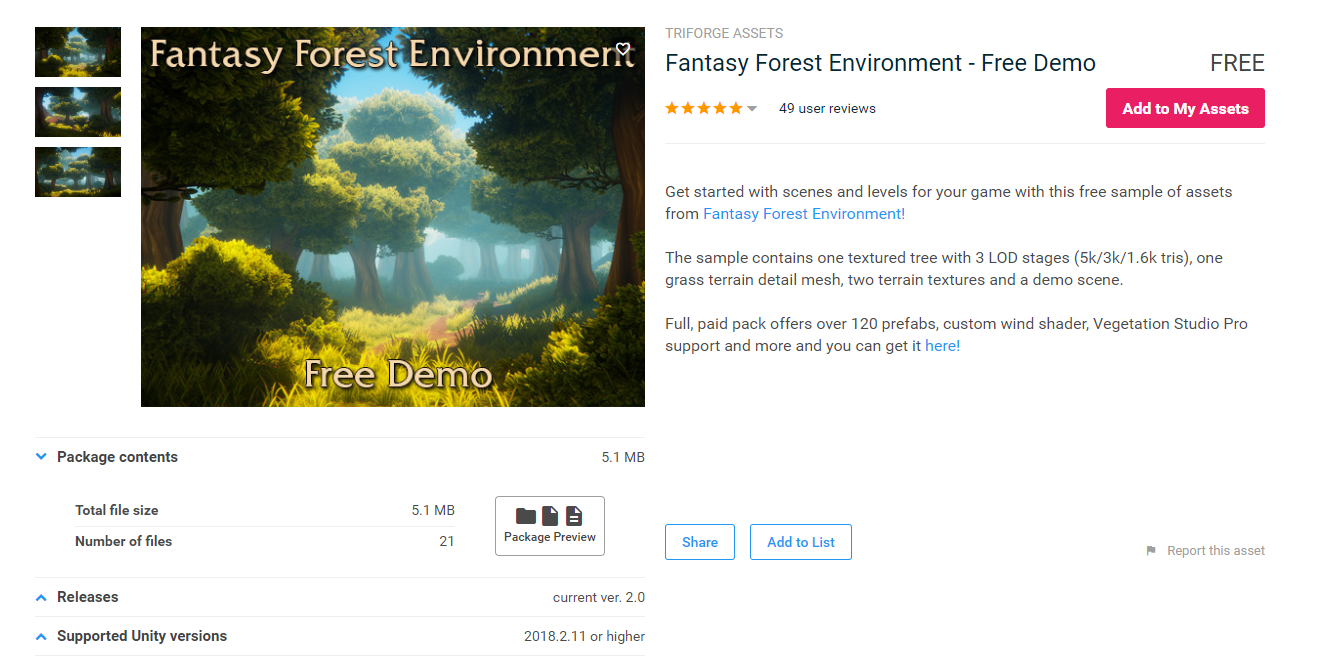
\includegraphics[width=0.7\textwidth]{./imagenes/fantasyForest}
	\caption{Fantasy Forest}
\end{figure} 

\quad El segundo asset ha sido descargado exclusivamente por el modelado de las estatuas, las cuáles han sido integradas al terreno en el que el jugador se sitúa. 

\begin{figure}[htb]
	\centering
	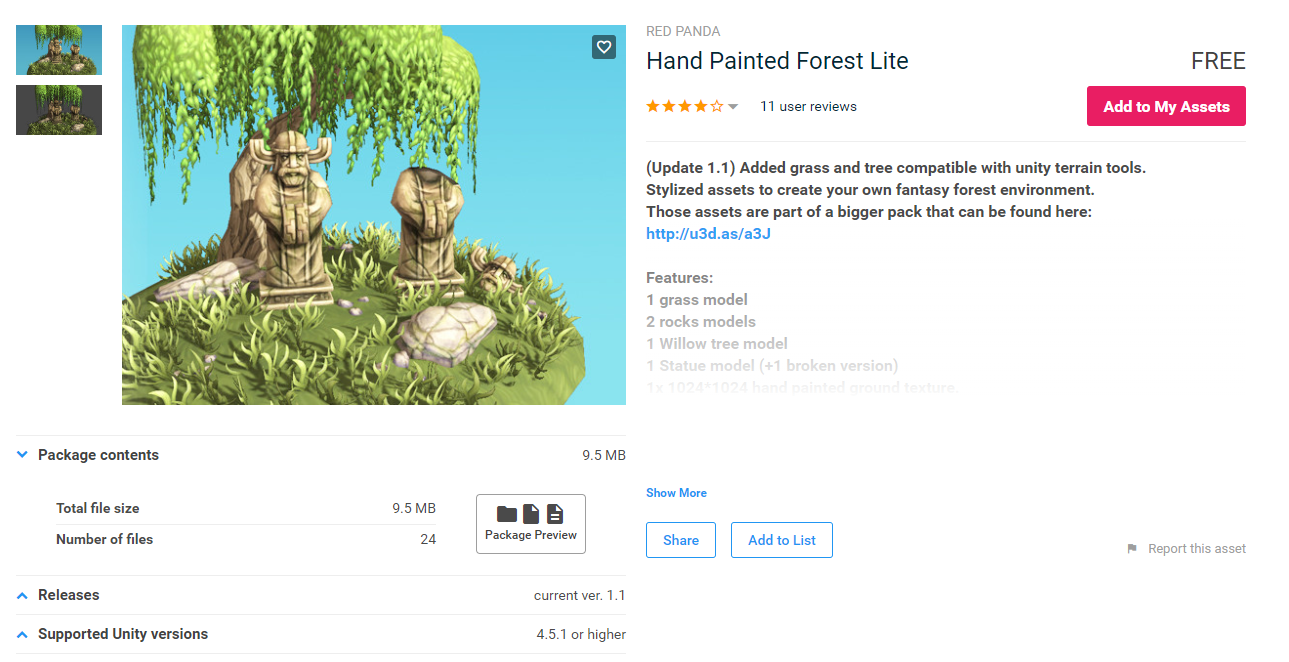
\includegraphics[width=0.7\textwidth]{./imagenes/handPaintedForest}
	\caption{Hand Painted Forest Lite}
\end{figure} 

\quad Este último asset pose los modelados y animaciones de los pajáros, ademas de un sistema para hacer que los pájaros se generaran automáticamente para simular un entorno órgánico. en el momento en el que se utizó este asset, lo unico implementado fuero los modelages con sus animaciones, ya que la mayoría de script asociados a la generación automática estaban vacíos, o directamente no existían, por lo que parte del desarrollo se dedicó a reacer gran parte de este asset.

\begin{figure}[htb]
	\centering
	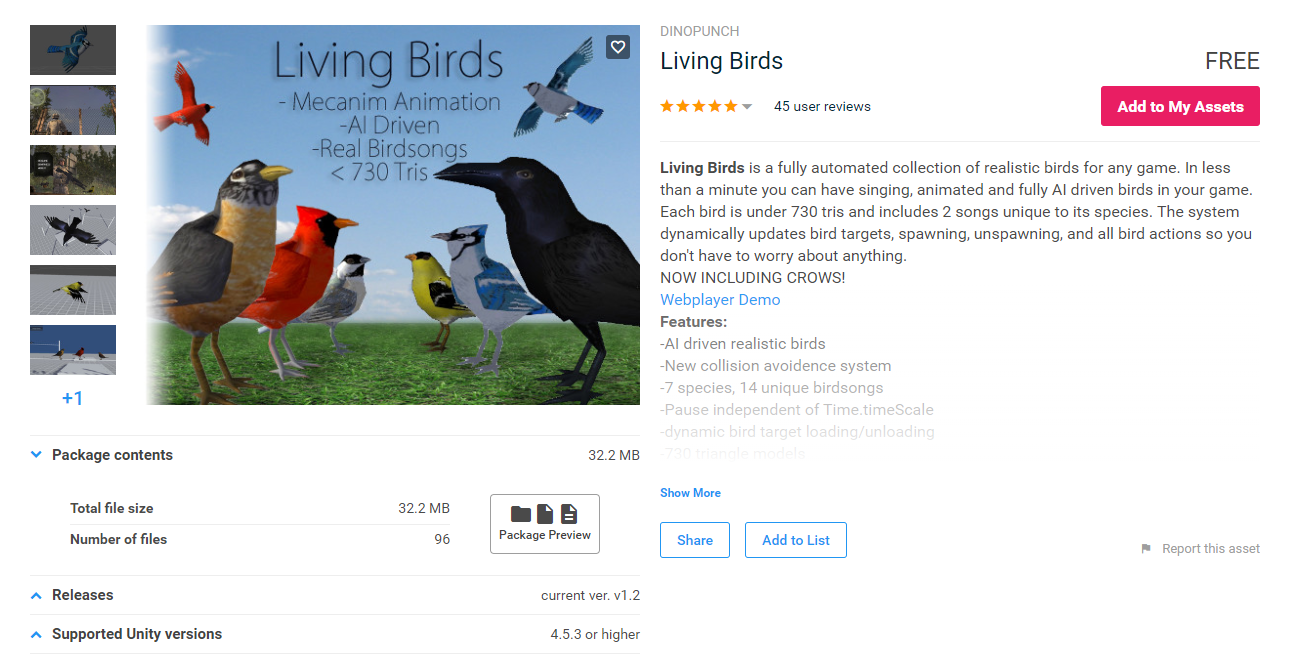
\includegraphics[width=0.7\textwidth]{./imagenes/livingBirds}
	\caption{Living Birds}
\end{figure} 

\subsection{Jugador}

\quad El jugador estará formado por un GameObject llamado \textit{RealPlayer} que contendrá la "MainCamera". Se introducirá como hijo de ésta el prefab \textit{GvrReticlePointer} que pondrá en el jugador la reticula que utilizaremos para las iteracciones. Hay una serie de cambios en la retícula que se explican en el siguiente subapartado.\\

\begin{figure}[htb]
	\centering
	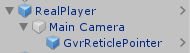
\includegraphics[width=0.8\textwidth]{./imagenes/player}
	\caption{Aspecto del Jugador en el árbol de escena}
\end{figure} 

\subsubsection{Controles de movimiento}

\quad Se ha implementado para el movimiento que cuando se hace click en la pantalla, el jugador se mueve. Esto se consigue añadiendo un script de C\# a \textit{RealPlayer} que contendra el siguiente código:

\lstset{language=[sharp]C, breaklines=true, basicstyle=\footnotesize}
\begin{lstlisting}[frame=single, caption={PlayerWalk.cs}]
using System.Collections;
using System.Collections.Generic;
using UnityEngine;

public class PlayerWalk : MonoBehaviour
{
    public int playerSpeed;

    // Update is called once per frame
    void Update()
    {
        if (Input.GetButton("Fire1")) {
            transform.position = transform.position + Camera.main.transform.forward * playerSpeed * Time.deltaTime;
        }
    }
}
\end{lstlisting}

\subsubsection{Control de cámara en VR}

\quad Simplemente se añadirá al árbol de escena el prefab de GoogleVR \textit{GvrEditorEmulator}.

\subsubsection{Retícula}

\quad La retícula que viene por defecto en unity no será necesaria en el caso presentado, pues es mejor y más eficiente utilizar el script \textit{GvrPointerPhysicsRaycaster.cs}, adjunto con el paquede de GoogleVR.\\

\quad La retícula es el medio para interactuar con el medio, pero no interesa que se active automáticamente, si no que será preciso que haya un tiempo de espera para que el usuario decida si se va a llevar a cavo esta interacción o si por el contrario desea canscelarla.\\

\quad Con motivo de ello, se aprobechará la capacidad de la retícula de google de ampliarse en una iteracción (efecto producido con el prefab \textit{GvrEventSystem}.) y se modificará el angulo mostrado en pantalla de ésta el cuál se irá modificando, convirtiendola así en una barra de carga circular. Para esto se requieren las siguientes modificaciones en el shader de Google:

\begin{itemize}
	\item Añadir la propiedad Angle
	\item Añadir el float que la representará
	\item Sustituir la función \textit{vert} para para que tenga en cuenta esta nueva propiedad en el shader 
\end{itemize}

\quad A continuación se adjunta el resultado final para ver como debe quedar el código:

\lstset{language=[sharp]C, breaklines=true, basicstyle=\footnotesize}
\begin{lstlisting}[frame=single, caption={GvrReticleShader.shader}]
// Copyright 2015 Google Inc. All rights reserved.
//
// Licensed under the Apache License, Version 2.0 (the "License");
// you may not use this file except in compliance with the License.
// You may obtain a copy of the License at
//
//     http://www.apache.org/licenses/LICENSE-2.0
//
// Unless required by applicable law or agreed to in writing, software
// distributed under the License is distributed on an "AS IS" BASIS,
// WITHOUT WARRANTIES OR CONDITIONS OF ANY KIND, either express or implied.
// See the License for the specific language governing permissions and
// limitations under the License.

Shader "GoogleVR/Reticle" {
  Properties {
    _Color  ("Color", Color) = ( 1, 1, 1, 1 )
    _InnerDiameter ("InnerDiameter", Range(0, 10.0)) = 1.5
    _Angle("Angle", Range(0, 360)) = 180
    _OuterDiameter ("OuterDiameter", Range(0.00872665, 10.0)) = 2.0
    _DistanceInMeters ("DistanceInMeters", Range(0.0, 100.0)) = 2.0
  }

  SubShader {
    Tags { "Queue"="Overlay" "IgnoreProjector"="True" "RenderType"="Transparent" }
    Pass {
      Blend SrcAlpha OneMinusSrcAlpha, OneMinusDstAlpha One
      AlphaTest Off
      Cull Back
      Lighting Off
      ZWrite Off
      ZTest Always

      Fog { Mode Off }
      CGPROGRAM

      #pragma vertex vert
      #pragma fragment frag

      #include "UnityCG.cginc"

      uniform float4 _Color;
      uniform float _InnerDiameter;
      uniform float _OuterDiameter;
      uniform float _DistanceInMeters;
      uniform float _Angle;

      struct vertexInput {
        float4 vertex : POSITION;
      };

      struct fragmentInput{
          float4 position : SV_POSITION;
      };

  /*    fragmentInput vert(vertexInput i) {
        float scale = lerp(_OuterDiameter, _InnerDiameter, i.vertex.z);

        float3 vert_out = float3(i.vertex.x * scale, i.vertex.y * scale, _DistanceInMeters);

        fragmentInput o;
        o.position = UnityObjectToClipPos (vert_out);
        return o;
      }
*/
      fragmentInput vert(vertexInput i) {
	  fragmentInput o;
	  if (_DistanceInMeters < 20) {
		  // 180* = 2.9
		  // limit = - (a - 180) * 2.9/180
		  float limit = -(_Angle - 180) * 0.0161111111;
		  float3 vert_out = float3(0, 0, _DistanceInMeters);
		  float a = -atan2(i.vertex.x, i.vertex.y);
		  if (a >= limit) {
			  float scale = lerp(_OuterDiameter, _InnerDiameter, i.vertex.z);
			  vert_out = float3(i.vertex.x * scale, i.vertex.y * scale, _DistanceInMeters);
		  }
		  o.position = UnityObjectToClipPos(vert_out);
	  }
	  return o;
}

      fixed4 frag(fragmentInput i) : SV_Target {
        fixed4 ret = _Color;
        return ret;
      }

      ENDCG
    }
  }
}

\end{lstlisting}

\subsubsubsection{Interacción de la retícula}

\quad Ahora entra en juego como conseguir la interacción con el objeto. Para ello se requieren dos pasos muy importantes: \\

\begin{itemize}
	\item Añadir al objeto un \textit{EventTrigger} que trabajará cuando el puntero entre dentro del area que ocupa el objeto y cuando salga.
	\item Añadir un script al objeto que en este caso se ha llamdo \textit{GVRButton.cs}.
\end{itemize}

\quad lo primero debe hacerle para determinar las fundiones GvrOn y GvrOff que determinarán el comportamiento ante la entrada y la salida del objeto. El segundo determina la acción que se llevará a cabo a partir de que termine el evento de entrada, que en este caso que la barra de carga termine de llenarse.\\

\quad Se adjuntan seguidamente es aspecto de un objeto que posee estas cualidades y el código asociado a \textit{GVRButton.cs}.\\

\lstset{language=[sharp]C, breaklines=true, basicstyle=\footnotesize}
\begin{lstlisting}[frame=single, caption={GVRButton.cs}]
using System.Collections;
using System.Collections.Generic;
using UnityEngine;
using UnityEngine.UI;
using UnityEngine.Events;

public class GVRButton : MonoBehaviour
{
    //public GameObject pointer;
    GameObject pointer;
    public UnityEvent GVRClick;
    public float totalTime = 2;
    bool gvrStatus;
    public float gvrTimer;
    Renderer rend;
    float angle;
    bool counted;

    private void Start()
    {
        pointer = GameObject.FindWithTag("gvrpointer");
        rend = pointer.GetComponent<Renderer>();
        counted = false;
    }

    // Update is called once per frame
    void Update()
    {
        if (gvrStatus)
        {
            gvrTimer += Time.deltaTime;
            angle = gvrTimer / totalTime * 360;
            rend.material.SetFloat("_Angle", angle);
        }

        if (gvrTimer > totalTime)
        {
            GVRClick.Invoke();
            gvrStatus = false;
        }
    }

    public void GvrOn()
    {
        gvrStatus = true;
    }

    public void GvrOff()
    {
        gvrStatus = false;
        gvrTimer = 0;
        rend.material.SetFloat("_Angle", 360f);
    }

    public void checkBird(string bird)
    {
        if (!counted)
        {
            GameObject.FindWithTag(bird).GetComponent<Text>().text = "OK";
            counted = true;
        }
    }
}

\end{lstlisting}

\begin{figure}[htb]
	\centering
	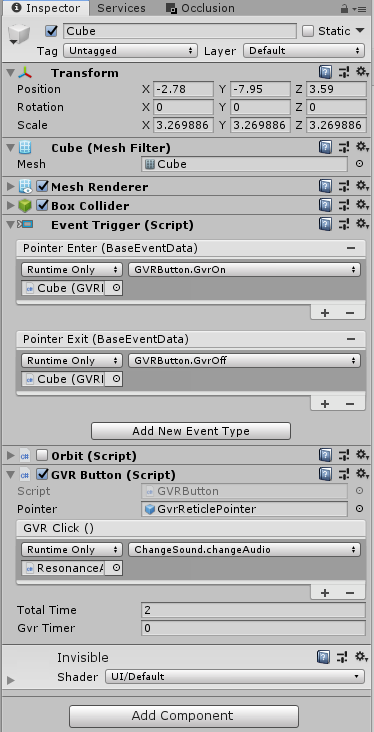
\includegraphics[width=0.35\textwidth]{./imagenes/cube}
	\caption{Cubo con interacciones}
\end{figure} 

\quad En el código se muestra como acceder al shader y modificar el ángulo que creamos en el apartado anterior dentro de la función update.\\

\subsubsection{Aplicar sonido 8D a un objeto}

\quad Esta parte se soluciona rápidamente añadiendo los dos siguientes elementos al objeto emisor de sonido y a la mainCamera:\\

\begin{itemize}
	\item El script \textit{ResonanceAudioListener.cs} a la main camera de la escena.
	\item El prefab\textit{ResonanceAudioSource} al objeto que hará de emisor.
\end{itemize}

\quad Es importante añadir el audio que queremos que se reproduzca en la propiedad \textit{Audio Source} para que los scripts puedan trabajar.

\begin{figure}[htb]
	\centering
	
\includegraphics[width=0.5\textwidth]{./imagenes/icosaedronHiche}
	\caption{Icosaedro con sonido en la gerarquía de escena}
\end{figure} 

\begin{figure}[htb]
	\centering
	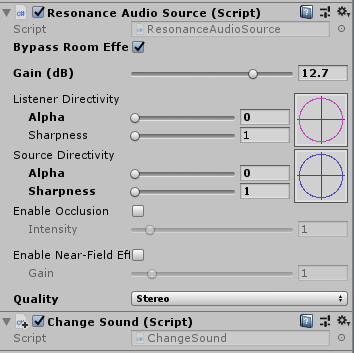
\includegraphics[width=0.5\textwidth]{./imagenes/audiosource}
	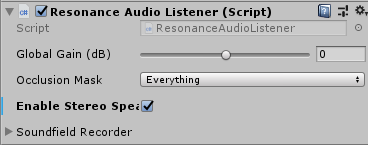
\includegraphics[width=0.5\textwidth]{./imagenes/audiolistener}
	\caption{Script ResonaceAudioSource y ResonanceAudioListener en el Inspector}
\end{figure} 

\subsection{Implementación por escenas}

\quad Ahora analizaremos los detalles más importantes implementados por escena.\\
 
	\subsubsection{Escena Init}
		\subsubsubsection{Cubo para interactuar}

\quad Ya se ha hablado de el cubo de la pimera escena que interactua con el usuario cuando lo mira, pero tiene varias acciones que realizar en el momento de la iteracción:

\begin{itemize}
	\item Cambiar el audio que se esta reproduciendo durante la ejecución.
	\item Cambiar la escena en la que se encuentra el jugador.
	\item Cambiar el material del cubo para que se haga visible.
\end{itemize}

\quad La primera acción requiere que por nuestra parte creemos un script que active la subrutina que cambie en ejecución el audio reproducido. La segunda accíon requiere que cuando se termine de reproducir el nuevo audio se cargue la siguiente escena. El siguiente código muestra como hacer ambas cosas desde la subrutina WaitFinish:\\

\lstset{language=[sharp]C, breaklines=true, basicstyle=\footnotesize}
\begin{lstlisting}[frame=single, caption={ChangeSound.cs}]
using System.Collections;
using System.Collections.Generic;
using UnityEngine;
using UnityEngine.SceneManagement;
using UnityEngine.Timeline;

public class ChangeSound : MonoBehaviour
{
    AudioSource myaudio;
    Material mymaterial;
    Renderer rend;

    public void changeAudio()
    {
        mymaterial = Resources.Load<Material>("RedMat");
        rend = GetComponentInParent<Renderer>();
        rend.enabled = true;
        rend.sharedMaterial = mymaterial;
        StartCoroutine(WaitFinish());
    }

    IEnumerator WaitFinish()
    {
        myaudio = GetComponent<AudioSource>();
        //myaudio.Stop();
        myaudio.clip = Resources.Load<AudioClip>("porfinteveo3");
        myaudio.Play();
        yield return new WaitForSeconds(myaudio.clip.length);
        SceneManager.LoadScene("EcoChamber");
    }
}

\end{lstlisting}

\quad En el mismo código se incluye dentro de la función changeAudio el método para poder cambiar el material de un GameObject.\\

	\subsubsection{Escena Echo Chamber}
		\subsubsubsection{Aplicar eco}
\quad Dentro del GameObject que define la habitación se debe añadir el prefab ResonanceAudioRoom, modificando el tamaño de este para que se ajuste al tamaño de la habitación.

\begin{figure}[htb]
	\centering
	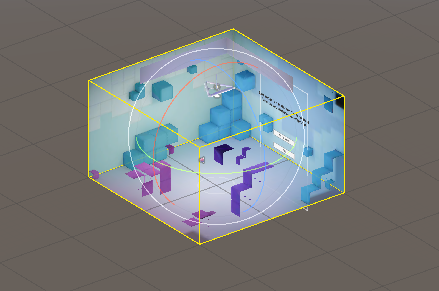
\includegraphics[width=0.55\textwidth]{./imagenes/echoroom}
	\caption{ResonanceAudioRoom ajustado a la habitación de la escena}
\end{figure} 

\quad Desde el script asociado al prefab, se pueden modificar los materiales que componen las dicerentes caras del cubo que delimita el espacio que dispondrá de eco, así como las características del eco en cuestión (reflectividad, tiempo, ganancia en DB, brillo).

\begin{figure}[htb]
	\centering
	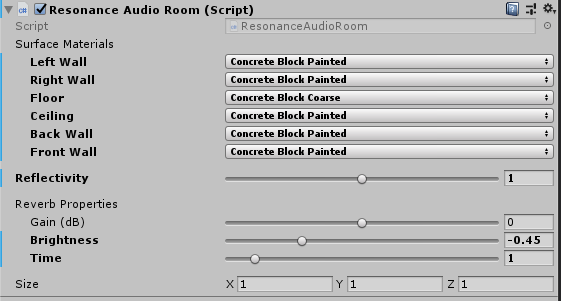
\includegraphics[width=0.55\textwidth]{./imagenes/audioroom}
	\caption{Script ResonaceAudioRoom}
\end{figure}

		\subsubsubsection{Cambiar en escena los materiales de la habitación}

\quad En la aplicación se encuentran varios materiales implementados para los diferentes lados del cubo que delimita la zona. Para simplificarlo, en esta aplicación solo se han implimentado una pequeña porción para demostrar un ejemplo de cambio de material dinámico de estos.\\ 

\quad La implementación de \textit{dropdown} ha sido llevada a cabo mediante el objeto suminstrado por Unity. Debido a que no se dispone de una version de pago para el desarrollo de esta aplicación, no se pueden tocar internamente el script que lo pone en funcionamiento, pero hay total libertad a la hora de añadir lo elementos que se requieran en la implementación.\\

\quad Siquiendo ese razonamiento, durante este desarrollo se han añadido un \textit{eventTrigger} y el escript anteriormente mencionado \textit{GVRButton}, haciendo la configuración requerida para poder interactuar con los elementos internos del dropdown.\\

\begin{figure}[htb]
	\centering
	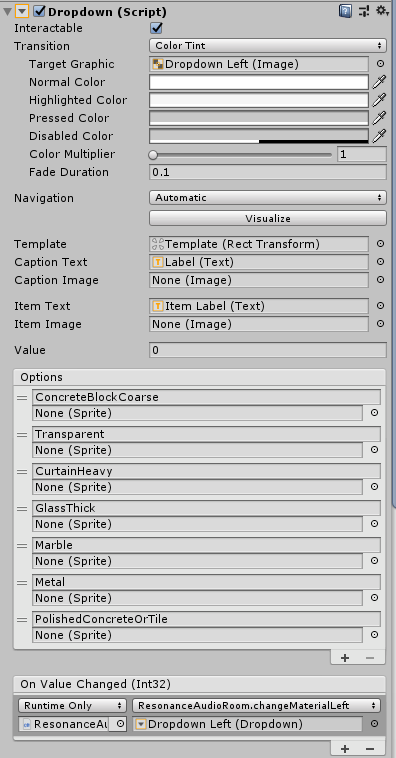
\includegraphics[width=0.4\textwidth]{./imagenes/dropDownScriptUnity}
	\caption{Script de un dropdown}
\end{figure}

\newpage
\quad Como se puede apreciar, no hay problema a la hora de definir los elementos del desplegable, a los que se les asignara por defecto un valor entero en el orden en el que son añadidos.\\ 

\begin{figure}[htb]
	\centering
	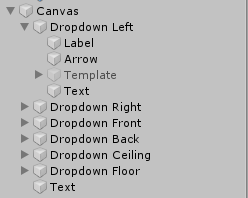
\includegraphics[width=0.5\textwidth]{./imagenes/dropdown}
	\caption{Dropdown en la gerarquía de escena}
\end{figure}

\quad Para poder acceder al valor asignado, en la zona de \textit{OnValueChage} se ha añadido al elemento \textit{ResonanceAudioRoom} como GameObject, y se llama a una de las funciones que se montaran dentro de su propio código llamadas \textit{changeMaterialRight}, \textit{changeMaterialLeft}, \textit{changeMaterialFront}, \textit{changeMaterialBack}, \textit{changeMaterialCeiling} y \textit{changeMaterialFloor}.\\

\begin{figure}[htb]
	\centering
	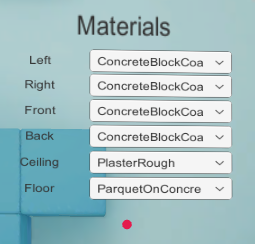
\includegraphics[width=0.3\textwidth]{./imagenes/materialMenu}
	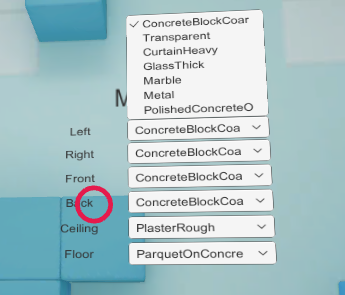
\includegraphics[width=0.4\textwidth]{./imagenes/materialMenuDeploy}
	\caption{Menú de cambio de material}
\end{figure} 

\newpage

\quad La implementación de las seis funciones mencionadas es prácticamente la misma, ya que solo se varía la referenciala lado sobre el que se vana  hacer las modificaciones.\\

\lstset{language=[sharp]C, breaklines=true, basicstyle=\footnotesize}
\begin{lstlisting}[frame=single, caption={Función changeMaterialRight}]
...
public ResonanceAudioRoomManager.SurfaceMaterial rightWall =
      ResonanceAudioRoomManager.SurfaceMaterial.ConcreteBlockCoarse;
...
public void changeMaterialRight(Dropdown mine)
    {
        int value = mine.value;

        switch (value)
        {
            case 0:
                rightWall = ResonanceAudioRoomManager.SurfaceMaterial.ConcreteBlockCoarse;
                break;
            case 1:
                rightWall = ResonanceAudioRoomManager.SurfaceMaterial.Transparent;
                break;
            case 2:
                rightWall = ResonanceAudioRoomManager.SurfaceMaterial.CurtainHeavy;
                break;
            case 3:
                rightWall = ResonanceAudioRoomManager.SurfaceMaterial.GlassThick;
                break;
            case 4:
                rightWall = ResonanceAudioRoomManager.SurfaceMaterial.Marble;
                break;
            case 5:
                rightWall = ResonanceAudioRoomManager.SurfaceMaterial.Metal;
                break;
            case 6:
                rightWall = ResonanceAudioRoomManager.SurfaceMaterial.PolishedConcreteOrTile;
                break;
            default:
                break;
        }
    }

\end{lstlisting}


		\subsubsubsection{Icosaedro el sonido}

\quad Respecto al icosaedro solo queda añadir la función que lo hace teleportarse cuando el evento entra en acción. Esta función se recoge en el siguiente código:\\

\lstset{language=[sharp]C, breaklines=true, basicstyle=\footnotesize}
\begin{lstlisting}[frame=single, caption={Teleporter.cs}]
using System.Collections;
using System.Collections.Generic;
using UnityEngine;

public class Teleporter : MonoBehaviour
{

    Vector3 destination;
    RectTransform rt;
    
    public void randomPlace()
    {
        destination = new Vector3(Random.Range(-8, 8), Random.Range(1, 8), Random.Range(-8, 8));
        rt = GetComponent<RectTransform>();
        rt.transform.localPosition = destination;
    }
}
\end{lstlisting}

	\subsubsection{Escena Forest}
		\subsubsubsection{Oclusion Culling}
\quad Occlusion Culling es una característica que desactiva el renderizado de objetos cuando actualmente no estén visibles por la cámara puesto que están oscurecidos (occluded) por otros objetos. Esto no sucede automáticamente en gráficas computacionales 3D ya que la mayoría de veces los objetos que están más lejos de la cámara son dibujados primero y los objetos más cercanos son dibujados encima de estos (esto se llama “overdraW”). El Occlusion Culling es diferente del Frustum Culling, ya que este solamente desactiva los renderers para objetos que están fuera del área visible de la cámara, pero no desactiva nada oculto de la vista por overdraw.\\

\quad Para que el culling funcione, los objetos que se deseenver afectados por él deben tener la casilla Static activada. De esta forma evitamos que objetos que se mueben se vean afectados por la desaparición en el dibujado.\\

\begin{figure}[htb]
	\centering
	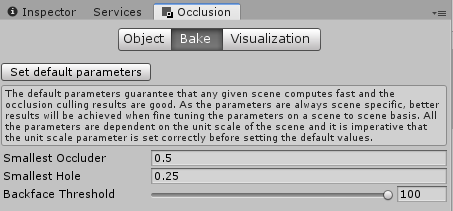
\includegraphics[width=1\textwidth]{./imagenes/cullingdata}
	\caption{Parametros aplicados en la aplicación para el culling}
\end{figure}

\begin{figure}[htb]
	\centering
	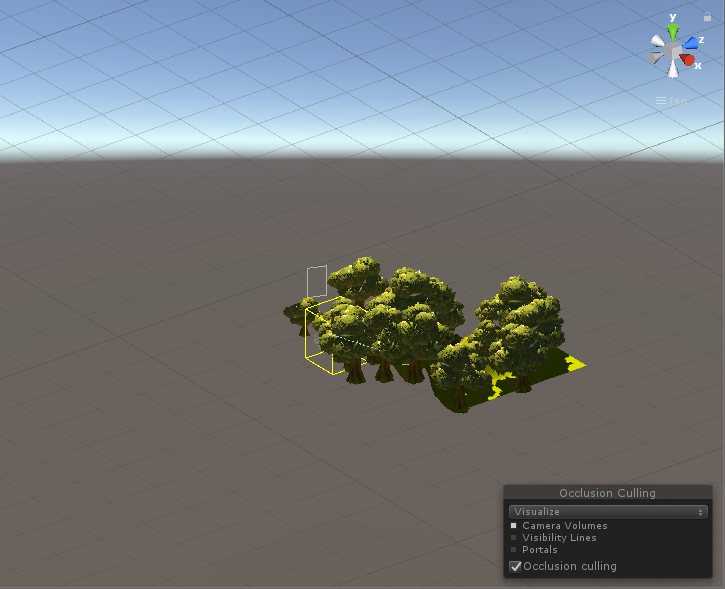
\includegraphics[width=0.40\textwidth]{./imagenes/culling1}
	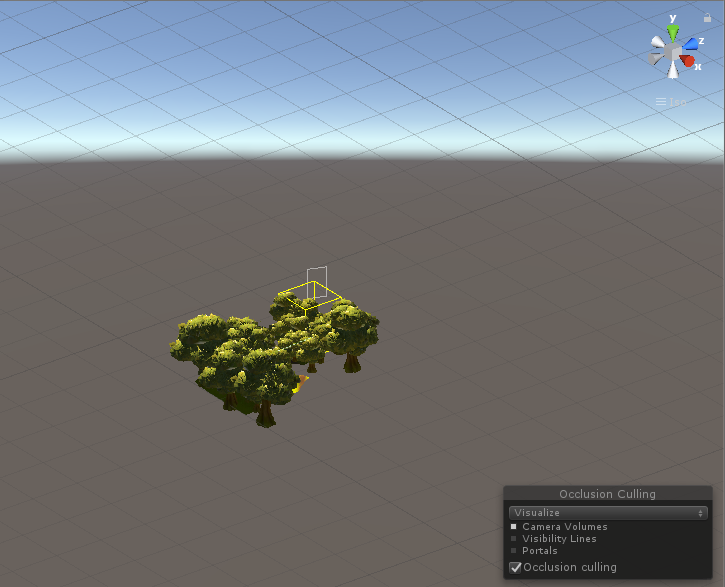
\includegraphics[width=0.40\textwidth]{./imagenes/culling2}
	\caption{Script ResonaceAudioRoom}
\end{figure}

		\subsubsubsection{Pájaros y su búsqueda}

\quad El sonido en los pájaros se genera de la misma forma que en cualquier elemento con sonido (el cubo o el icosaedro), aunque presentan una pequeña diferencia. Donde encontremos dentro del script \textit{lb\_Bird.cs} una reproducción de uno de los cuatro audios que componen los sonidos del pájaro, se debe tener en cuenta que ahora el pájaro no contará con un AudioSource propio, si no que ese componente se encontrará dentro del objeto hijo ResonanceAudioSource que se le añadirá.\\

\quad Para poder acceder al componente de este onjeto hijo, se debera cambiar la linea que hace el play por lo siguiente:\\

\lstset{language=[sharp]C, breaklines=true, basicstyle=\footnotesize}
\begin{lstlisting}[frame=single, caption={Ejemplo de cambio de audio para pájaro}]
	this.transform.Find("ResonanceAudioSource").gameObject.GetComponent<AudioSource>().PlayOneShot (song1,1);
\end{lstlisting}

\quad Deben hacerse cuatro cambios en el script \textit{lb\_Bird.cs}.\\

\quad Lo último a tener en cuenta en esta escena, es cambiar el shader de los materiales que componen la escena a \textit{Movile/Diffuse}. De esta forma se garantiza que el shader está optimizado para trabajar en un móvil.\\

\quad Ahora toca la implementación para poder interactuar con los distitos pájaros que aparecen en la escena, de forma que cuando interactuemos con dentro de la lista \textit{Most Wanted!!} situada encima del menú en el bosque, esta chequee a ese ave en particular y la marque con un \textit{OK}.\\ 

\quad Con ese fin se ha escrito dentro del script GVRButton la función checkBird, a la cual se le pasa un string, el cual será el tag del texto que deberemos cambiar de vacío a "OK".\\

\begin{lstlisting}[frame=single, caption={función checkBird}]
public void checkBird(string bird)
    {
        if (!counted)
        {
            GameObject.FindWithTag(bird).GetComponent<Text>().text = "OK";
            counted = true;
        }
    }
\end{lstlisting}

\quad Es importante recordar que hay que modificar el prefad de cada pajaro que se queira convertir en interactuable mediante los pasos que ya se explicaron con anterioridad.\\


\newpage



